\documentclass[oneside, 10pt]{article}

\usepackage{amsmath}
\usepackage{amsfonts}
%\usepackage{algorithm}
%\usepackage{algorithmic}
\usepackage{multirow}
\usepackage{colortbl}
\usepackage{color}
\usepackage[table]{xcolor}
\usepackage{epigraph}
%\usepackage{subfigure}
\usepackage{caption}
\usepackage{subcaption}
\usepackage{tabularx}
\usepackage{float}
\usepackage{longtable}
\usepackage[pdftex]{graphicx}
\usepackage{pdfpages}
\usepackage{tabularx}
\usepackage{pdflscape}
\usepackage[acronym,toc]{glossaries}
\usepackage[margin=1.2in]{geometry}

\usepackage[style=ieee,backend=biber]{biblatex}
\addbibresource{report.bib}


\providecommand{\tightlist}{%
	\setlength{\itemsep}{0pt}\setlength{\parskip}{0pt}}
\setcounter{secnumdepth}{0}

\PassOptionsToPackage{hyphens}{url} % url is loaded by hyperref
\usepackage[unicode=true]{hyperref}

\setlength{\parindent}{0pt}
\setlength{\parskip}{6pt plus 2pt minus 1pt}


\title{Opinion Mining and Social Media Sentiment Analysis in the Prediction of Cryptocurrency Prices}
\date{Submission date: Place Holder}
\author{Student: Andrew Sotheran
	\\Student Number: fr005432
	\\Supervisor: Kenneth Boness
	\\Word Count: Place Holder}

\begin{document}
	
	\maketitle
	
	\vspace*{\fill}
	\begin{center}
		\section{Abstract}\label{abstract}
	\end{center}
		The volatility of the stock markets is an aspect that is both hard to predict and to mitigate especially when relating to the cryptocurrency market. Cryptocurrency is highly volatile and which has attracted investors to attempt to make quick profits on the market.

	
	\newpage
	\begin{center}
		\section{Acknowledgements}\label{acknowledgements}
	\end{center}
	
	\newpage
	\begin{center}
		\section{Glossary}\label{glossary}
	\end{center}
	Bull(ish)/Bear(ish) Markets - Relates to a trend of the market price increasing and decreasing respectively
	
	Highs/Lows - The highest and lowest trading price of a giving period
	
	Fiat Currency - A currency without intrinsic value that has been established as money
	
	BTC - Bitcoin's stock symbol
	
	Twitter - Online social media platform, which allows users to post information or express opinions through messages called "Tweets"
	
	Tweets - The name given for messages posted on the Twitter platform, which are restricted to 280 characters.
	
	\newpage
	
	\begin{center}
		\tableofcontents
	\end{center}
	
	\newpage
	\begin{center}
		\section{Introduction}\label{introduction}
	\end{center}
	The premise of this project is to investigate into whether the sentiment in social media has a correlation to the prices of cryptocurrencies and how this could be used to predict future changes in the price. 
	
	The chosen cryptocurrency that will be focused in this project will be the currency that has the most community and backing and has been known to lead other fiat currencies, Bitcoin (BTC). Bitcoin is seen as one, if not the first cryptocurrency to bring a wider following to the peer-to-peer token transaction scene since 2009. Although it was not the first token to utilise blockchain technology, it allowed investors to openly trade a public cryptocurrency which provided pseudonymous means of transferring funds through the internet. Thus it has been around longer than most of the other fiat currencies and is the most popular crypto-token due to it's larger community base.
	
	Most financial commodities are subject to the whim of public confidence and are the core of it's base value. A platform that is frequently used for the public to convey their opinions on a commodity is that of Twitter which provides arguably biased information and opinions. Whether the opinions present a basis in facts or not, they are usually taken at face value and can influence the public opinion of given topics. As Bitcoin has been around since 2009 the opinions and information on the commodity are prevalent through the platform. 
	In the paper \textit{Sentiment Analysis of Twitter Data for Predicting Stock Market Movements} by \textit{Majhi et al.} \cite{1} 2.5 million tweets on Microsoft were extracted from Twitter, sentiment analysis and logistical regression performed on the data yielded 69.01\% accuracy for a 3-day period on the increase/decrease in stock price. These results showed a "\textit{good correlation between stock market movements and the sentiments of public expressed in Twitter}".
	
	The background of this project is in response to the volatility of the cryptocurrency market, which can fluctuate at a moments notice and can be seen to be social media driven. The history of the price of Bitcoin and what was being discussed on the currency around it's most volatile period to-date, Nov-2017 to Feb-2018, shows a strong bullish trend which saw Bitcoin reach a \$19,500 high in mid-Dec. While social media, such as Twitter, during that period was had an extremely positive outlook on the cryptocurrency. The trend was short lived and saw the market crash only a month later, with only a couple of sell-offs, expected for the holidays rush, accompanied by negative outlooks posted on social media turned the market against itself which saw the longest bearish market in Bitcoin's history and is still trying to recover today.
	
	Due to how volatile the crypto-market can be, there is a need to either mitigate or to anticipate where the markets are heading. As the crypto-market and Bitcoin are affected by socially constructed opinions, either through Twitter, news articles or other forms of media, there is a way to perform the latter, where the prices of Bitcoin could be predicted based on the sentiment gathered from social media outlets.
	
	The aim of this project is to create a tool that gathers tweets from Twitter, obtains the overall sentiment score of the given text while gathering historical price data for the time period gathering occurs. Features are then extracted from the gathered data and used in a neural network to ascertain whether the price of the currency can be predicted from the correlation between the sentiment and price history of the data.
	
	This report will discuss the justifications for the project and the problems it will be attempting to resolve, the stakeholders that would benefit the most from this system and what this project will not attempt to accomplish. Similar tools will be critiqued and examined for their feature set and credibility in the literature review along with current sentiment analysers, algorithms, natural language processing techniques and neural networks in their respective topics and comparing their accuracy for this project purpose. 
	The solution approach will discuss the decisions and reasoning behind choosing the techniques and tools used for this project and will outline the requirements for this project.
	Implementation of the chosen techniques and tools, with the discussion of important functions of the system will formulate the implementation section of this report with an in-detail explanation of the function's use and data flow of the system.
	
	\newpage
	
	\begin{center}
		\section{Problem Articulation}\label{problem}
	\end{center}
		
		\subsection{Problem Statement}\label{statement}
		
		The key problems this project will attempt to address are that of a public open-source system that aids in the analysis and prediction of BTC, the accuracy of open-source tools and technology when applied to trading market scene and to identify whether there is a correlation between Twitter sentiment and BTC price fluctuation. While there are tools out there only a few are available to the public and only provide basic functionality such as only sentiment analysis, while others are kept in-house of major corporations whom invest into this problem domain.
		
		The other issue presented here is that assuming perfect accuracy can be achieved is naive. As this project will only be using existing tools and technologies thus, there are limitations to accuracy that can be obtained. One of that being the suitability of the tools, there are no open-source sentiment analysers for stock market prediction thus finding a specifically trained analyser for the chosen domain in highly unlikely. In relation, finding the most suitable machine learning or neural network is equally important as this will determine the accuracy of the predictions.
		
		The accuracy and suitability of various machine learning methods and neural networks are a known issue in their respective domains, this investigation should be carried out to determine their suitability for their needed use in this project.
		
		This project will focus on the investigation of these technologies and whether it is feasible to predict the price of BTC based on historical price and the sentiment gathered from Twitter. The accuracy of the system will be compared to other technologies to identify limitations in the proposed solution and to determine the for other technologies if this is the case. 
		
		A system will be created that will utilise  
		
		\subsection{Stakeholders}\label{stakeholders}
		
		\subsection{Project Constraints}\label{constraints}
	
	\newpage
	
	\begin{center}
		\section{Literature Review}\label{literature}
	\end{center}
			\subsection{Existing Tools}
			
			\subsection{Related Work}
			
			\subsection{Tweet Collection}\label{tweet_collection}
		
			\subsection{Sentiment Analysis}\label{sentiment}
	
			\subsubsection{Algorithms}\label{algorithms}
			\subsubsection{Techniques}\label{techniques}
			
		\subsection{Neural Networks}\label{networks}
			\subsubsection{Types}\label{types}
			\subsubsection{LSTMs}\label{lstms}
		
		\subsection{Machine Learning}\label{machine}
			\subsubsection{Logistical Regression}
		
	\newpage
	
	\begin{center}
		\section{Solution Approach}\label{solution}
	\end{center}
	
		\subsection{Solution Summary}\label{sumary}
		
		\subsection{Data flow Overview}\label{data-flow}
		
		\subsection{Packages, Tools and Techniques}\label{tools}
		
	\newpage
	
	\begin{center}	
		\section{System Design and Implementation}\label{implementation}
	\end{center}
		\subsection{Data collection}\label{collection}
		
		\subsection{Data processing}\label{processing}
			\subsubsection{Preprocessing}
				\paragraph{Tweet Filtering}
				\paragraph{Text Cleaning}
				\paragraph{Ngram based Language detection filtering}
			
			\subsubsection{Spam Filtering}
				\paragraph{Tweet Processing}
				\paragraph{Naive Bayes model}
				\paragraph{Multinomial Naive Bayes}
				\paragraph{Bernoullis Naive Bayes}
				\paragraph{Gaussuan Naive Bayes}
		
		\subsection{Sentiment Analysis}
			\subsubsection{VADER}
			
	\newpage
	
	\section{Testing: Verification and Reflection}
	
	\newpage
	
	\section{Discussion: Contribution and Reflection}
	\subsection{Limitations}
	
	\newpage
	
	\section{Social, Legal and Ethical Issues}
	
	\newpage
	
	\section{Conclusion and Future Improvements}
		\subsection{Conclusion}
		\subsection{Future Improvements}
		
	\newpage
	
	\section{References}
	\nocite{*}
	\printbibliography
	
	\newpage
	\section{Appendices}
		\subsection{Appendix A - Project Initiation Document}
		Displayed on the following pages below.
		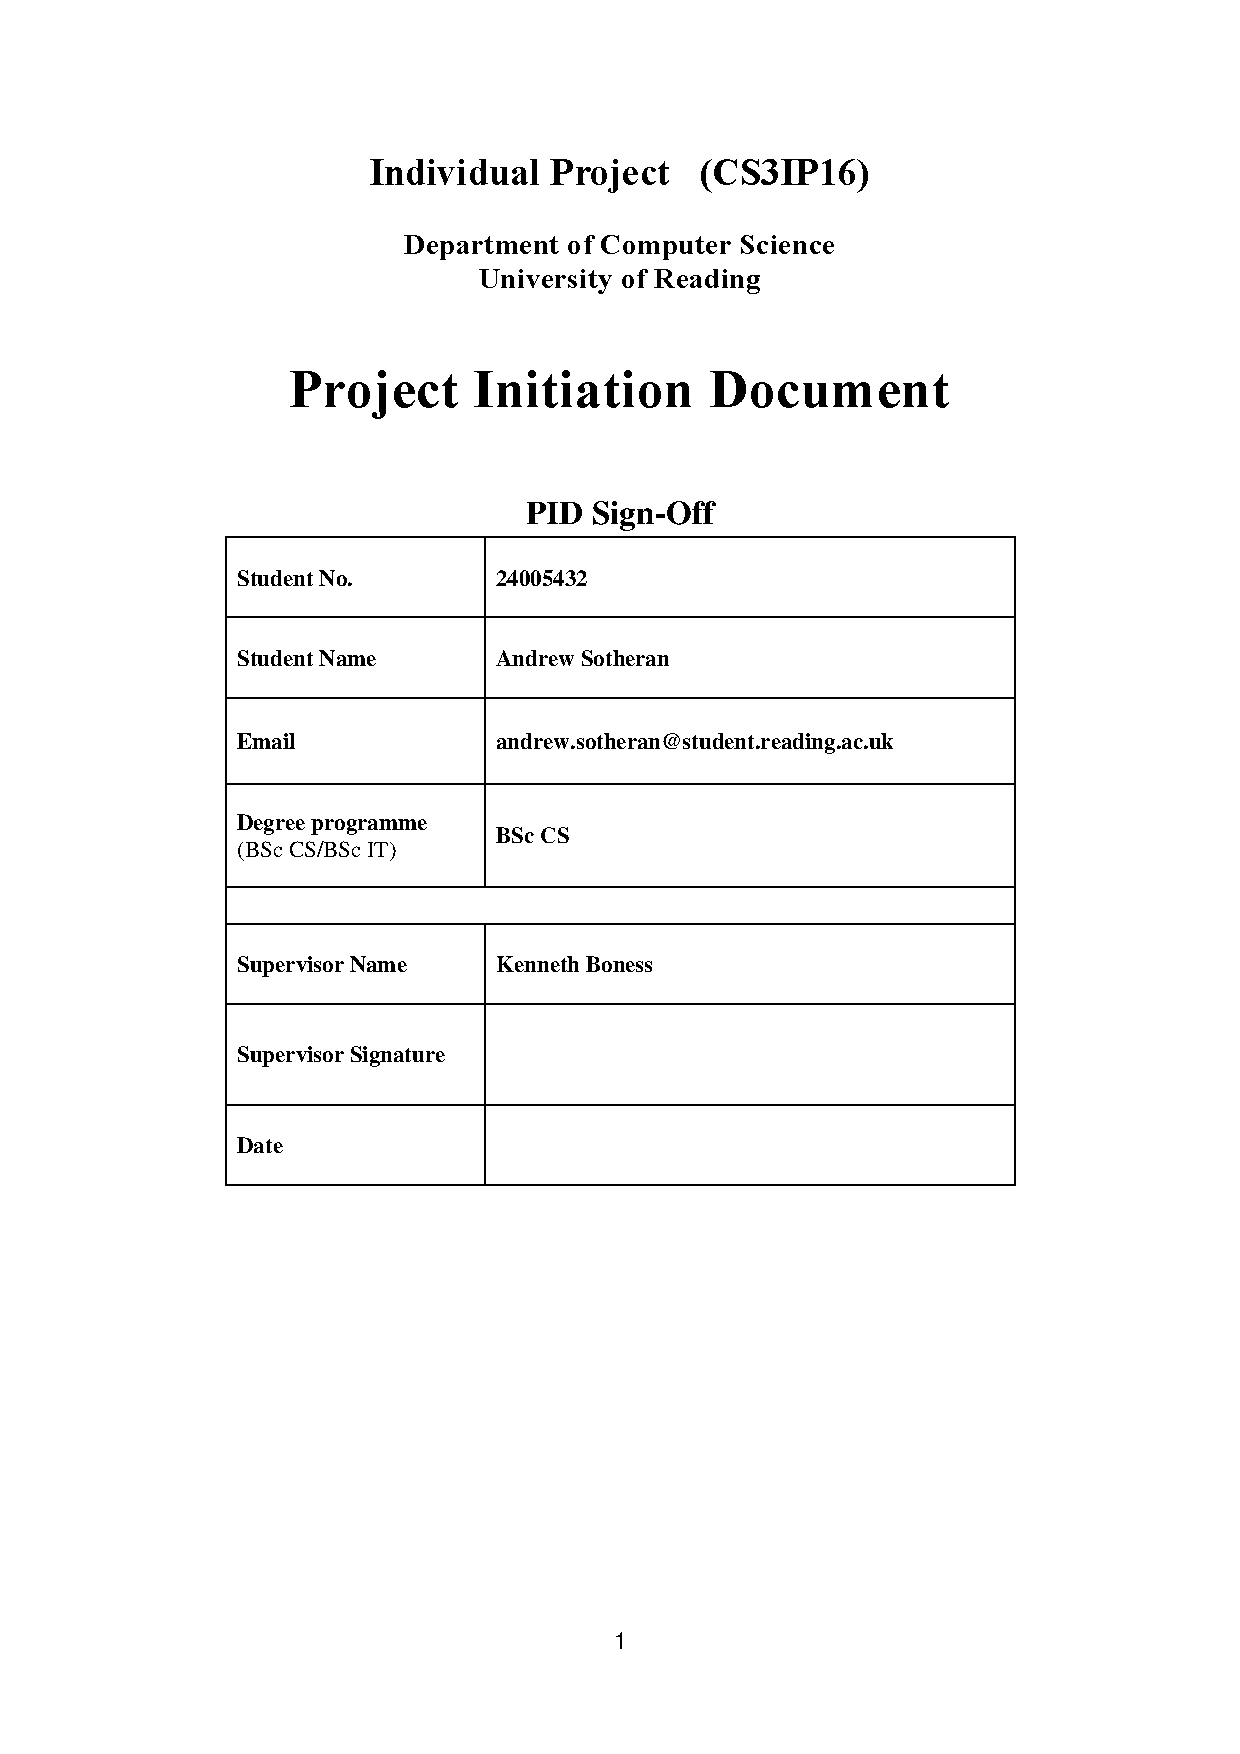
\includepdf[pages=-]{PID}
		\subsection{Appendix B - Log book}
		The log book for this project is a physical book and was handed to the School of Computer Science. Due to being a physical book, it cannot be inserted here.
	
\end{document}